\documentclass[conference]{IEEEtran}
\IEEEoverridecommandlockouts
% The preceding line is only needed to identify funding in the first footnote. If that is unneeded, please comment it out.
\usepackage{cite}
\usepackage{amsmath,amssymb,amsfonts}
\usepackage{algorithmic}
\usepackage{array}
\usepackage{graphicx}
\usepackage{textcomp}
\usepackage{xcolor}
\usepackage{microtype}
\usepackage{tikz}
\usetikzlibrary{arrows.meta,positioning,shapes.geometric,fit}
\def\BibTeX{{\rm B\kern-.05em{\sc i\kern-.025em b}\kern-.08em
    T\kern-.1667em\lower.7ex\hbox{E}\kern-.125emX}}
\begin{document}

\title{Smart Warehouse AI Agent: Document Understanding and Inventory Anomaly Decision Agent
\thanks{TODO: Identify applicable funding agency here, or remove this footnote if none.}
}

\author{\IEEEauthorblockN{TODO: Author Information}
\IEEEauthorblockA{\textit{TODO: Department / School Name} \\
\textit{TODO: Organization / University Name}\\
TODO: City, Country \\
TODO: Email Address or ORCID}
}

\maketitle

\begin{abstract}
Warehouse digitization does not automatically ensure reliable inventory data. Although warehouse management systems are widely adopted, front-end document intake, field verification, and exception handling still rely heavily on manual effort, and isolated optical character recognition (OCR) pipelines cannot verify whether an inbound, outbound, or cycle-count document conflicts with inventory state or domain policies. Conversely, allowing unconstrained large language models to trigger inventory mutations introduces hallucination, non-reproducibility, and authorization risks. We present the Smart Warehouse AI Agent, an evidence-first, recommendation-only, and human-gated domain agent architecture connecting unstructured warehouse documents to auditable inventory anomaly decisions. The proposed eight-module design separates bounded task planning from deterministic OCR, schema parsing, read-only SQLite retrieval, quantity reconciliation, versioned warehouse rules, and human confirmation with append-only auditing. We explicitly distinguish current implementation from planned work: a local Python, SQLite, and Streamlit minimum viable prototype (MVP) has been built with a rule-based bounded planner, synthetic and optional Tesseract OCR adapters, exact document-number duplicate checking, stock-availability verification, and confirmation-before-write auditing, passing six automated synthetic integration tests. However, dynamic LLM-assisted replanning, scanned-PDF rendering, Google Sheets retrieval, fuzzy duplicate matching, calibrated risk-coverage gating, and the planned 300-to-500-document three-baseline benchmark remain unexecuted.
\end{abstract}

\begin{IEEEkeywords}
warehouse document understanding, inventory anomaly detection, domain AI agent, evidence-based reasoning, human-in-the-loop, optical character recognition
\end{IEEEkeywords}

\section{Introduction}

\subsection{Motivation and Problem Context}
Warehouse operations rely on accurate synchronization between physical goods movements and digital inventory records across receiving, put-away, order picking, shipping, and cycle counting. In the 2025 Warehouse/DC Operations Survey ($n = 101$ qualified respondents), 87\% of surveyed facilities reported using a warehouse management system (WMS), yet 51\% still collected productivity data manually, 76\% tracked inventory accuracy as a key metric, and average stock-keeping unit (SKU) counts grew from 7,790 to 9,565~\cite{b12}. Although this industry survey is non-peer-reviewed and cannot be extrapolated globally, it highlights a persistent gap between system adoption and reliable front-end data automation. Empirical supply-chain studies further show that inventory record inaccuracy (IRI) degrades operational control and fulfillment performance~\cite{b15,b16,b19}, and can arise from scanning omissions, unit mismatches, and process errors even when automated visibility technologies are deployed~\cite{b17,b18}.

At the document intake boundary, receiving notes, shipping orders, cycle-count sheets, and logistics labels arrive as images, PDFs, or spreadsheets containing heterogeneous vendor layouts. Standardized logistics labeling guidelines such as GS1 specify identifiers including Serial Shipping Container Codes (SSCC), Global Trade Item Numbers (GTIN), counts, batch/lot numbers, and dates to preserve traceability~\cite{b11}. However, raw Optical Character Recognition (OCR) outputs character strings and local confidence scores without verifying whether a document number has already been posted, whether requested outbound quantities exceed available stock, whether SKUs exist in master data, or whether inventory snapshots are stale. Fixed rule scripts validate known formats but fail brittlely under missing fields, layout drift, or cross-source conflicts, whereas unconstrained Large Language Models (LLMs) risk generating unsupported claims or executing unauthorized state changes.

\subsection{Related Work and Research Gap}
Prior work spans two largely parallel streams: Document AI and Smart Warehousing. In Document AI, SROIE~\cite{b4} established a benchmark of 1,000 scanned receipts for text localization, OCR, and key information extraction (KIE), and DocVQA~\cite{b5} framed document understanding as visual question answering over 12,000+ images and 50,000 questions; however, neither dataset models external inventory state, domain rules, or operational approval gates. Principe et al.~\cite{b3} compared human annotation, rule-based methods, and LLM extraction on real-estate auction documents, demonstrating accuracy, maintainability, and cost trade-offs rather than universal LLM superiority. Recent agentic document frameworks---AID-Agent~\cite{b2}, evaluated on 44 annotated industrial technical PDFs, and DocAgent~\cite{b1}, which uses hierarchical outlines, interactive page retrieval, and a reviewer agent---demonstrate the value of domain tools and cross-checking, but do not address warehouse inventory reconciliation or write-permission safety.

In warehouse domain research, recent systematic reviews highlight that IoT warehousing studies remain largely theoretical with limited field deployment~\cite{b6}, call for unified integration across cyber-physical systems, digital twins, SKU flows, and human-centric KPIs~\cite{b9}, and synthesize AI-enhanced digital twin applications including anomaly detection~\cite{b10}. Rad et al.~\cite{b8} combined order simulation with stakeholder interviews for AI-based batch picking, showing that organizational and workflow fit govern adoption alongside algorithmic gains. Xu et al.~\cite{b7} reported an inventory anomaly detection ensemble achieving 87.3\% F1 on 12,358 SKUs in e-commerce data; however, only the abstract and registry metadata have been verified to date, leaving data splits, anomaly definitions, and baseline comparisons unverified (marked TODO) and unsuitable as a direct baseline here. Meanwhile, governance standards such as NIST AI RMF 1.0~\cite{b13} and its Generative AI Profile~\cite{b14} emphasize data quality, provenance, traceability, and risk-calibrated human oversight.

Synthesizing these lines reveals a research gap: the lack of a lightweight, evidence-first domain AI agent that bridges unstructured bilingual warehouse documents to read-only inventory retrieval, versioned domain rules, and human-gated recommendations, together with a controlled comparison against manual workflows and fixed OCR-rule pipelines. Note that an exhaustive systematic search log confirming global novelty remains pending (TODO). Additional citations on Chinese/bilingual warehouse OCR benchmarks and human automation-bias studies in review interfaces are also needed (TODO).

\subsection{Research Questions and Contributions}
This study investigates four measurable research questions (RQs):
\begin{itemize}
    \item \textbf{RQ1 (Document Understanding):} Under unseen vendor templates and image degradation, how accurately does the pipeline extract key fields (document number, date, warehouse, pallet type, SKU, quantity, and unit), measured by Character Error Rate (CER), Field Exact Match (EM), and Document EM?
    \item \textbf{RQ2 (Anomaly Decision):} When combining extracted fields with read-only inventory snapshots, document history, and versioned domain rules, how effectively does the agent detect duplicates, missing critical fields, unknown SKUs, invalid quantities/units, insufficient stock, and warehouse mismatches?
    \item \textbf{RQ3 (Agent Value):} Compared with manual processing (B0) and fixed OCR + rules (B1), does the bounded agent (B2) improve task completion, tool selection, processing time, or human workload without increasing false auto-acceptance?
    \item \textbf{RQ4 (Trustworthiness):} Can the system ground material claims in traceable evidence IDs, escalate under low confidence, stale snapshots, or source conflicts, and support append-only audit replay?
\end{itemize}

The intended contributions---all pending full empirical validation beyond the current MVP---are: (C1) framing warehouse document verification as a bounded, risk-gated document-to-decision problem; (C2) an eight-module, recommendation-only architecture isolating deterministic tools from agent orchestration; (C3) a paired three-baseline evaluation protocol with template-group splitting; and (C4) a reproducible local-first Python/SQLite prototype.

\section{System Design}

\subsection{Design Principles and Responsibility Boundaries}
The architecture follows five core principles derived from domain analysis and risk governance~\cite{b11,b13,b14}: (1) \textit{process and state conservation}, verifying transactions against prior inventory states; (2) \textit{end-to-end provenance}, linking extracted fields and findings back to source spans and database rows; (3) \textit{fitness for use}, separating field confidence, completeness, conflict, and snapshot freshness rather than relying on a single average score; (4) \textit{exception-based human gating}, keeping formal WMS writes out of agent scope; and (5) \textit{closed-loop root-cause separation}, distinguishing observed anomalies from hypothesized causes without silent overwrites.

Crucially, the design enforces strict responsibility boundaries:
\begin{itemize}
    \item \textbf{Planner / Agent:} Maps task intent, selects allowlisted retrieval and analysis tools, detects missing context, and structures evidence-linked rationales without inventing SKUs, quantities, or rules, and without storing hidden chain-of-thought.
    \item \textbf{Deterministic Modules:} Execute file validation, schema parsing, date/decimal/unit normalization, parameterized read-only SQL queries, exact duplicate key matching, quantity conservation, hard warehouse rules, and the final human gate.
    \item \textbf{Statistical Modules (Target Design):} Compute OCR confidence aggregation, numeric deviations, fuzzy duplicate candidates (never treated as confirmed facts), outlier scores, and latency metrics.
    \item \textbf{Human Operator:} Performs approve, edit, reject, or reprocess actions for flagged or high-risk cases with recorded actor identity and reasons.
\end{itemize}

\subsection{Eight-Module Architecture and Processing Flow}
The target system comprises eight numbered modules, illustrated in Fig.~\ref{fig:architecture}:
\begin{enumerate}
    \item \textbf{User / Application Scenario:} Defines operator role, warehouse context, and workflow intent (\texttt{RECEIPT}, \texttt{ISSUE}, or \texttt{CHECK}), rejecting unauthorized contexts.
    \item \textbf{Query / Input:} Accepts natural-language task queries and PNG, JPEG, or PDF files, computes a SHA-256 file hash, assigns a \texttt{trace\_\allowbreak id}, and rejects empty, corrupted, or oversized inputs.
    \item \textbf{Planner \& Reasoning Agent:} Validates task intent against an allowed scenario list and constructs a step-bounded plan restricted to an explicit tool allowlist.
    \item \textbf{Data Acquisition / Retrieval:} Performs preprocessing, OCR extraction (returning spans, bounding boxes, and confidences), typed schema parsing, and read-only lookups against inventory, document history, and master data.
    \item \textbf{Analytics Engine:} Normalizes dates, \texttt{Decimal} quantities, and units; separates exact duplicate keys from fuzzy candidates; checks quantity conservation and snapshot freshness; and computes evidence coverage.
    \item \textbf{Domain Knowledge Integration:} Evaluates versioned warehouse rules and item control policies (e.g., GS1 identifiers, unit validity, pallet types, conditional batch/expiry rules).
    \item \textbf{Decision / Recommendation:} Combines rule severities, confidence, evidence coverage, conflicts, and freshness into finite dispositions (\texttt{PASS\_\allowbreak RECOMMENDED}, \texttt{FLAG\_\allowbreak ANOMALY}, \texttt{REQUEST\_\allowbreak CORRECTION}, \texttt{HUMAN\_\allowbreak REVIEW\_\allowbreak REQUIRED}, or \texttt{BLOCK\_\allowbreak RECOMMENDED}).
    \item \textbf{Output \& Interaction:} Displays source evidence alongside findings in Streamlit, enforces human confirmation before writing test records, and logs append-only audit events.
\end{enumerate}

The target execution flow (Algorithm~1 in the project specification and Fig.~\ref{fig:flowchart}) proceeds from file validation and trace initialization to bounded planning, OCR with at most one alternate-preprocessing retry, deterministic normalization and critical-field validation, read-only database retrieval with freshness checks, duplicate and reconciliation analytics, versioned rule evaluation, an unsupported-claim blocker, risk-confidence-coverage gating, and human review with bounded reprocess attempts. Five execution invariants govern the flow: \texttt{NO\_\allowbreak WMS\_\allowbreak WRITE}, \texttt{NO\_\allowbreak UNSUPPORTED\_\allowbreak CLAIM}, \texttt{NO\_\allowbreak SILENT\_\allowbreak CORRECTION}, \texttt{BOUNDED\_\allowbreak EXECUTION}, and \texttt{FAIL\_\allowbreak SAFE}.

\begin{figure*}[t]
\centering
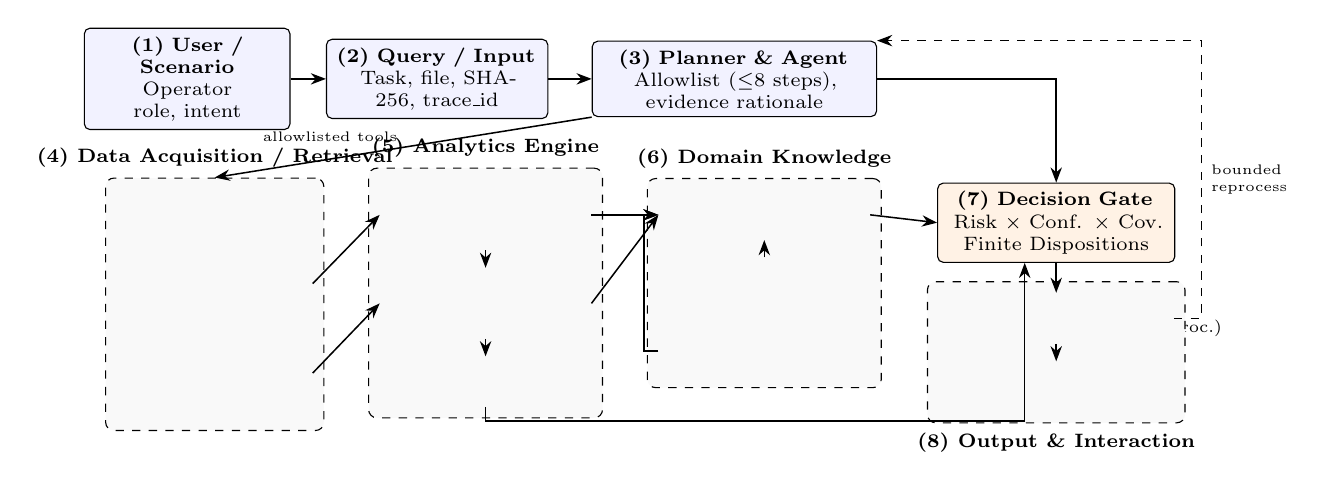
\begin{tikzpicture}[
    font=\scriptsize,
    >=Stealth,
    mod/.style={draw, rounded corners=2pt, align=center, fill=blue!5, minimum height=0.82cm, inner sep=3pt},
    sub/.style={draw, rounded corners=2pt, align=center, fill=white, minimum height=0.62cm, inner sep=2.5pt, font=\fontsize{6.5}{7.5}\selectfont},
    grp/.style={draw, dashed, rounded corners=3pt, inner sep=4pt, fill=gray!5},
    gate/.style={draw, rounded corners=2pt, align=center, fill=orange!10, minimum height=0.82cm, inner sep=3pt},
    arr/.style={->, line width=0.55pt}
]
% Top intake and planner row
\node[mod, text width=2.4cm] (m1) {\textbf{(1) User / Scenario}\\Operator role, intent};
\node[mod, text width=2.6cm, right=0.45cm of m1] (m2) {\textbf{(2) Query / Input}\\Task, file, SHA-256, trace\_id};
\node[mod, text width=3.4cm, right=0.55cm of m2] (m3) {\textbf{(3) Planner \& Agent}\\Allowlist ($\le$8 steps), evidence rationale};

% Acquisition group (4)
\node[sub, text width=2.3cm, below=0.75cm of m1, xshift=0.35cm] (pre) {Preprocess \& OCR\\(spans, bbox, conf.)};
\node[sub, text width=2.3cm, below=0.22cm of pre] (parse) {Schema Parser\\(typed Document)};
\node[sub, text width=2.3cm, below=0.22cm of parse] (inv) {Read-Only Retrieval\\(SQLite / Sheets / Hist.)};
\node[grp, fit=(pre)(parse)(inv), label={[font=\scriptsize\bfseries]above:(4) Data Acquisition / Retrieval}] (g4) {};

% Analytics group (5)
\node[sub, text width=2.5cm, right=0.85cm of pre] (norm) {Normalize \& Exact/Fuzzy\\Duplicate Check};
\node[sub, text width=2.5cm, below=0.22cm of norm] (rec) {Stock Reconciliation \&\\Snapshot Freshness};
\node[sub, text width=2.5cm, below=0.22cm of rec] (stat) {Outlier Stats \&\\Evidence Coverage};
\node[grp, fit=(norm)(rec)(stat), label={[font=\scriptsize\bfseries]above:(5) Analytics Engine}] (g5) {};

% Domain Knowledge group (6)
\node[sub, text width=2.5cm, right=0.85cm of norm] (rules) {Versioned Warehouse\\Rule Engine};
\node[sub, text width=2.5cm, below=0.22cm of rules] (master) {Item Master, Batch,\\Expiry, Risk Class};
\node[sub, text width=2.5cm, below=0.22cm of master] (gs1) {GS1 Traceability\\(SKU, GTIN, SSCC)};
\node[grp, fit=(rules)(master)(gs1), label={[font=\scriptsize\bfseries]above:(6) Domain Knowledge}] (g6) {};

% Decision (7) and Output (8)
\node[gate, text width=2.8cm, right=0.85cm of rules, yshift=-0.1cm] (m7) {\textbf{(7) Decision Gate}\\Risk $\times$ Conf. $\times$ Cov.\\Finite Dispositions};
\node[sub, text width=2.8cm, below=0.38cm of m7] (rev) {Human Review Gate\\(Approve/Edit/Reject/Reproc.)};
\node[sub, text width=2.8cm, below=0.22cm of rev] (out) {Streamlit UI \&\\Append-Only Audit Log};
\node[grp, fit=(rev)(out), label={[font=\scriptsize\bfseries]below:(8) Output \& Interaction}] (g8) {};

% Connections
\draw[arr] (m1) -- (m2);
\draw[arr] (m2) -- (m3);
\draw[arr] (m3.south west) -- node[above left=-2pt, font=\tiny] {allowlisted tools} (g4.north);
\draw[arr] (parse.east) -- (norm.west);
\draw[arr] (inv.east) -- (rec.west);
\draw[arr] (norm) -- (rec);
\draw[arr] (rec) -- (stat);
\draw[arr] (norm.east) -- (rules.west);
\draw[arr] (rec.east) -- (rules.west);
\draw[arr] (master) -- (rules);
\draw[arr] (gs1.west) -- ++(-0.18,0) |- (rules.west);
\draw[arr] (stat.south) -- ++(0,-0.18) -| ([xshift=-0.4cm]m7.south);
\draw[arr] (rules.east) -- (m7.west);
\draw[arr] (m3.east) -| (m7.north);
\draw[arr] (m7) -- (rev);
\draw[arr] (rev) -- (out);
\draw[arr, dashed] (rev.east) -- ++(0.35,0) |- node[pos=0.25, right, font=\tiny, align=left] {bounded\\reprocess} (m3.north east);
\end{tikzpicture}
\caption{Eight-module evidence-first architecture separating bounded agent orchestration (Module~3) from deterministic acquisition, analytics, versioned rules, and human-gated output (Modules~4--8), adapted from \texttt{architecture.md}.}
\label{fig:architecture}
\end{figure*}

\begin{figure*}[t]
\centering
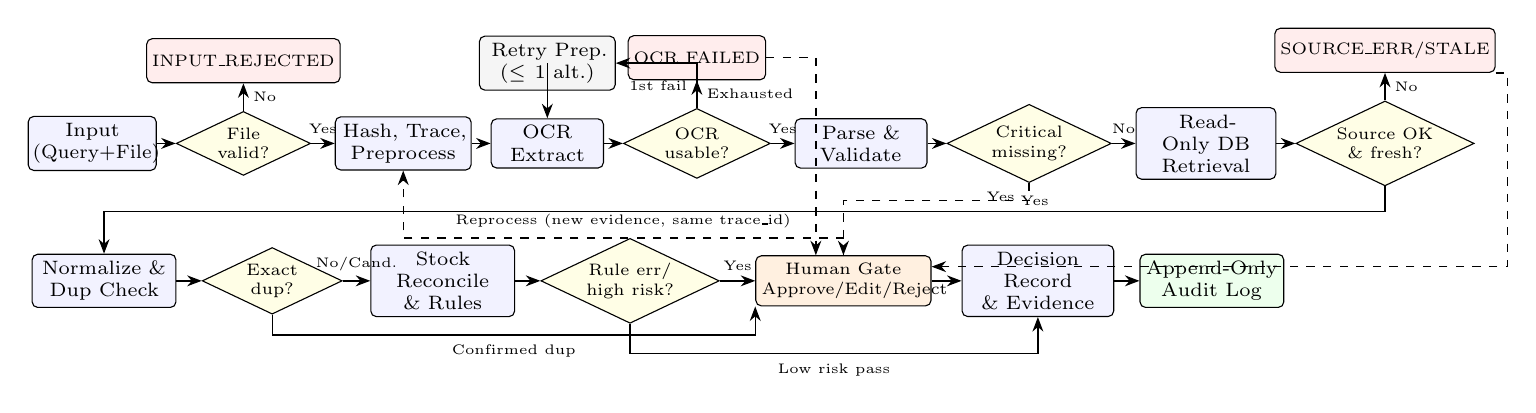
\begin{tikzpicture}[
    font=\scriptsize,
    >=Stealth,
    proc/.style={draw, rounded corners=2pt, align=center, fill=blue!5, minimum height=0.62cm, inner sep=2.5pt},
    dec/.style={draw, diamond, aspect=2.1, align=center, fill=yellow!10, inner sep=1pt, font=\fontsize{6}{7}\selectfont},
    exc/.style={draw, rounded corners=2pt, align=center, fill=red!7, minimum height=0.56cm, inner sep=2pt, font=\fontsize{6}{7}\selectfont},
    hum/.style={draw, rounded corners=2pt, align=center, fill=orange!12, minimum height=0.62cm, inner sep=2.5pt, font=\fontsize{6.5}{7.5}\selectfont},
    arr/.style={->, line width=0.5pt}
]
% Row 1: Intake -> OCR -> Schema -> Retrieval
\node[proc, text width=1.45cm] (in) {Input\\(Query+File)};
\node[dec, right=0.24cm of in] (vfile) {File\\valid?};
\node[proc, text width=1.55cm, right=0.30cm of vfile] (prep) {Hash, Trace,\\Preprocess};
\node[proc, text width=1.25cm, right=0.24cm of prep] (ocr) {OCR\\Extract};
\node[dec, right=0.24cm of ocr] (ook) {OCR\\usable?};
\node[proc, text width=1.50cm, right=0.30cm of ook] (parse) {Parse \&\\Validate};
\node[dec, right=0.24cm of parse] (miss) {Critical\\missing?};
\node[proc, text width=1.60cm, right=0.30cm of miss] (acq) {Read-Only DB\\Retrieval};
\node[dec, right=0.24cm of acq] (dsok) {Source OK\\\& fresh?};

% Exceptions above Row 1
\node[exc, above=0.35cm of vfile] (ein) {INPUT\_REJECTED};
\node[proc, text width=1.55cm, above=0.35cm of ocr, fill=gray!8] (retry) {Retry Prep.\\($\le 1$ alt.)};
\node[exc, above=0.35cm of ook] (ofail) {OCR\_FAILED};
\node[exc, above=0.35cm of dsok] (dfail) {SOURCE\_ERR/STALE};

% Row 2: Analytics -> Rules -> Decision -> Human -> Audit
\node[proc, text width=1.65cm, below=1.05cm of in, xshift=0.15cm] (ana) {Normalize \&\\Dup Check};
\node[dec, right=0.32cm of ana] (dup) {Exact\\dup?};
\node[proc, text width=1.65cm, right=0.35cm of dup] (rec) {Stock Reconcile\\\& Rules};
\node[dec, right=0.32cm of rec] (rerr) {Rule err/\\high risk?};
\node[hum, text width=2.05cm, right=0.45cm of rerr] (human) {Human Gate\\Approve/Edit/Reject};
\node[proc, text width=1.75cm, right=0.38cm of human] (out) {Decision Record\\\& Evidence};
\node[proc, text width=1.65cm, right=0.32cm of out, fill=green!7] (log) {Append-Only\\Audit Log};

% Row 1 arrows
\draw[arr] (in) -- (vfile);
\draw[arr] (vfile) -- node[right, font=\tiny] {No} (ein);
\draw[arr] (vfile) -- node[above, font=\tiny] {Yes} (prep);
\draw[arr] (prep) -- (ocr);
\draw[arr] (ocr) -- (ook);
\draw[arr] (ook) |- node[pos=0.25, left, font=\tiny] {1st fail} (retry);
\draw[arr] (retry) -| (ocr);
\draw[arr] (ook) -- node[right, font=\tiny] {Exhausted} (ofail);
\draw[arr] (ook) -- node[above, font=\tiny] {Yes} (parse);
\draw[arr] (parse) -- (miss);
\draw[arr] (miss) -- node[above, font=\tiny] {No} (acq);
\draw[arr] (acq) -- (dsok);
\draw[arr] (dsok) -- node[right, font=\tiny] {No} (dfail);

% Transition Row 1 -> Row 2
\draw[arr] (dsok.south) -- ++(0,-0.32) -| node[pos=0.15, above, font=\tiny] {Yes} (ana.north);

% Escalations to Human Gate
\draw[arr, dashed] (ofail.east) -| ([xshift=-0.35cm]human.north);
\draw[arr, dashed] (miss.south) -- ++(0,-0.22) -| node[pos=0.05, right, font=\tiny] {Yes} (human.north);
\draw[arr, dashed] (dfail.south east) -- ++(0.15,0) |- ([yshift=0.18cm]human.east);

% Row 2 arrows
\draw[arr] (ana) -- (dup);
\draw[arr] (dup) -- node[above, font=\tiny] {No/Cand.} (rec);
\draw[arr] (dup.south) -- ++(0,-0.26) -| node[pos=0.25, below, font=\tiny] {Confirmed dup} (human.south west);
\draw[arr] (rec) -- (rerr);
\draw[arr] (rerr) -- node[above, font=\tiny] {Yes} (human);
\draw[arr] (rerr.south) -- ++(0,-0.38) -| node[pos=0.25, below, font=\tiny] {Low risk pass} (out.south);
\draw[arr] (human) -- (out);
\draw[arr] (out) -- (log);
\draw[arr, dashed] (human.north) -- ++(0,0.22) -| node[pos=0.25, above, font=\tiny] {Reprocess (new evidence, same trace\_id)} (prep.south);
\end{tikzpicture}
\caption{Bounded execution and exception-handling flow corresponding to Algorithm~1 and \texttt{flowchart.md}, enforcing single-retry OCR preprocessing, fail-safe escalation, and append-only audit logging.}
\label{fig:flowchart}
\end{figure*}

\subsection{Implemented MVP vs. Planned Target Design}
To avoid conflating design specifications with completed software, Table~\ref{tab:impl_boundary} explicitly contrasts what is currently implemented in the repository against planned components. In particular, the current \texttt{RuleBasedPlanner} constructs a uniform seven-step plan across \texttt{RECEIPT}, \texttt{ISSUE}, and \texttt{CHECK} intents (within an eight-step cap and seven-tool allowlist), and \texttt{agent/llm.py} currently enforces an explicit disabled/not-implemented boundary. Accordingly, the present codebase is accurately characterized as an executable OCR/parser, deterministic rule, and bounded-orchestration MVP rather than a complete adaptive LLM agent.

\begin{table*}[t]
\caption{Implementation Boundary: Currently Implemented MVP vs. Planned Target Design}
\label{tab:impl_boundary}
\centering
\footnotesize
\setlength{\tabcolsep}{4pt}
\begin{tabular}{|>{\raggedright\arraybackslash}p{2.4cm}|>{\raggedright\arraybackslash}p{6.6cm}|>{\raggedright\arraybackslash}p{7.1cm}|}
\hline
\textbf{Subsystem} & \textbf{Implemented in Current MVP} & \textbf{Planned / Not Yet Implemented} \\
\hline
UI \& Input (\texttt{app.py}) & Streamlit upload and query UI; SHA-256 hash and UUID \texttt{trace\_\allowbreak id}; empty-file rejection; human confirmation checkbox and actor entry before test DB write. & Full interactive browser validation; multi-action human edit, reject, and bounded reprocess loop. \\
\hline
Planner (\texttt{agent/\allowbreak planner.py}) & \texttt{RuleBasedPlanner} mapping \texttt{RECEIPT}, \texttt{ISSUE}, \texttt{CHECK}; 7-tool allowlist; max 8 steps; generates fixed 7-step plan. & Dynamic state-dependent replanning on missing data or tool errors; schema-constrained LLM adapter (\texttt{agent/\allowbreak llm.py} raises \texttt{NotImplementedError}; note \texttt{OptionalLLMService.\allowbreak available()} polarity bug in audit). \\
\hline
OCR \& Parsing (\texttt{ocr/}) & \texttt{SyntheticOCRProvider} for UTF-8 fixtures; \texttt{pypdf} text-PDF extraction (untested automatically); \texttt{AutoOCRProvider} failing explicitly if Tesseract is missing; line-level evidence IDs. & Image rotation/denoising preprocessing; single automatic OCR retry; scanned-PDF page rendering; word-level bounding boxes and calibrated OCR confidences. \\
\hline
Retrieval (\texttt{database/}) & SQLite \texttt{documents} and \texttt{audit\_\allowbreak log} tables; synthetic inventory seeding; history lookup by \texttt{document\_\allowbreak no}; duplicate-write block. & Read-only production/Google Sheets adapter; separate master-data table; inventory \texttt{as\_\allowbreak of\_\allowbreak time} snapshot freshness tracking. \\
\hline
Analytics (\texttt{analytics/}) & Exact duplicate check by \texttt{document\_\allowbreak no}; \texttt{UNKNOWN\_\allowbreak SKU} check; \texttt{ISSUE} available-stock check (\texttt{on\_\allowbreak hand - reserved}). & Fuzzy duplicate candidate scoring; \texttt{Decimal} unit-conversion reconciliation; statistical outlier summaries; evidence coverage calculation. \\
\hline
Domain Rules (\texttt{domain/}) & Required fields (\texttt{document\_\allowbreak no}, \texttt{date}, \texttt{warehouse}, \texttt{pallet\_\allowbreak type}, items), positive quantity, allowed units (\texttt{PCS}, \texttt{BOX}, \texttt{EA}, Chinese unit tokens), allowed pallets. & Externalized versioned YAML/JSON policy repository with \texttt{rule\_\allowbreak id}, \texttt{source}, \texttt{version}, conditional batch/expiry rules, and conflict detection. \\
\hline
Decision \& Audit (\texttt{agent/\allowbreak service.py}) & Deterministic status (\texttt{PASS\_\allowbreak RECOMMENDED}, \texttt{REQUEST\_\allowbreak CORRECTION}, \texttt{HUMAN\_\allowbreak REVIEW\_\allowbreak REQUIRED} when findings exist or confidence $< 0.75$, \texttt{FAILED}); SQLite audit events. & Full \texttt{risk $\times$ confidence $\times$ coverage $\times$ freshness} decision table; unsupported-claim blocker; tamper-evident hash-chained JSONL audit ledger. \\
\hline
\end{tabular}
\end{table*}

\section{Experimental Setup}

\subsection{Dataset and Leakage-Controlled Splitting}
The planned evaluation uses a three-tier data strategy (currently \textbf{Not Run} / \textbf{TODO}):
\begin{enumerate}
    \item \textbf{Public Sanity Pretest:} SROIE~\cite{b4} and DocVQA~\cite{b5} only for OCR/KIE pipeline sanity checking, without claiming warehouse domain performance.
    \item \textbf{Main Bilingual Dataset (Planned):} 300--500 anonymized or synthetic Chinese/English warehouse documents covering at least three document types and five vendor templates.
    \item \textbf{Paired Operational Context (Planned):} Each document paired with an immutable SQLite inventory snapshot, item master data, document history, and adjudicated ground truth across eight label classes: normal, duplicate document, missing critical field, unknown SKU, invalid quantity/unit, insufficient stock, warehouse mismatch, and conditional batch/expiry missing.
\end{enumerate}

To prevent layout memorization leakage across splits, documents will be partitioned by \texttt{vendor\_\allowbreak id + template\_\allowbreak id} group split into 60\% train, 20\% validation, and 20\% test using \texttt{random\_\allowbreak seed = 20261024}, freezing manifest checksums prior to testing. Dual annotation with adjudication and data-card documentation remain TODO.

\subsection{Baselines and Fairness Controls}
Three baselines will be evaluated on the identical frozen test manifest, gold labels, and restored SQLite snapshots:
\begin{itemize}
    \item \textbf{B0 (Manual Entry and Verification):} Human operators read source documents, manually type key fields, query the same read-only database interface, and assign anomaly flags and dispositions without seeing B1/B2 outputs, using counterbalanced ordering.
    \item \textbf{B1 (OCR + Fixed Rules):} Executes a fixed sequential pipeline (\texttt{OCR $\rightarrow$ parse $\rightarrow$ query $\rightarrow$ duplicate check $\rightarrow$ rules $\rightarrow$ output}) sharing the exact OCR engine, preprocessing, parser, rule version, and thresholds as B2, with no adaptive planning.
    \item \textbf{B2 (OCR + Domain AI Agent):} Shares B1's underlying tools and deterministic decision gate while adding bounded task routing, allowlisted tool selection, and limited replanning or escalation under missing context, source conflicts, or tool failures.
\end{itemize}

\subsection{Evaluation Metrics and Statistical Protocol}
Evaluation covers document quality, anomaly detection, operational efficiency, and agent safety:
\begin{equation}
\mathrm{CER} = \frac{S + D + I}{N_{\mathrm{gold}}}, \quad \mathrm{CharAcc} = \max(0, 1 - \mathrm{CER}),
\end{equation}
where $S$, $D$, and $I$ denote character substitutions, deletions, and insertions, and $N_{\mathrm{gold}}$ is the gold character count (reported for B1/B2 OCR output and separately as manual transcription accuracy for B0). Key-field Exact Match (EM) and Document EM evaluate normalized values across document number, date, warehouse, pallet type, SKU, quantity, and unit. Multi-label anomaly detection uses one-vs-rest Precision, Recall, and F1 per class alongside macro-F1 (proposed primary endpoint, pending advisor confirmation; TODO). Duplicate detection reports both Duplicate Accuracy and Precision/Recall/F1, separating confirmed duplicates from fuzzy candidates. Operational metrics include mean, median, and P95 end-to-end processing time (including human review time for B2) and Human Intervention Rate. Agent-only metrics for B2 include Tool Selection Precision, Tool Selection Recall, Safe Tool Rate, Task Completion Rate, Evidence Coverage, Appropriate Escalation Rate, and False Auto-accept Rate. Planned primary comparison (B2 vs. B1) will use paired bootstrap 95\% confidence intervals, McNemar tests for paired binary outcomes, and Wilcoxon signed-rank tests for continuous latencies.

\section{Results}

\subsection{Observed Engineering Verification (MVP)}
Formal comparative experiments (B0, B1, B2) have \textbf{not been executed}. To date, only engineering verification of the synthetic-data MVP has been performed (recorded in the project audit and design documents under Python 3.11.9). Table~\ref{tab:mvp_tests} summarizes all verified checks. All six automated integration tests in \texttt{tests/\allowbreak test\_\allowbreak mvp.py} passed in 0.117\,s. These checks verify software execution paths and fail-safe behaviors on synthetic UTF-8 text fixtures only; they do \textbf{not} measure real-image OCR accuracy, scanned PDF handling, LLM reasoning, latency benchmarks, or agent superiority.

\begin{table}[t]
\caption{Observed Engineering Verification of the Current MVP}
\label{tab:mvp_tests}
\centering
\footnotesize
\setlength{\tabcolsep}{3pt}
\begin{tabular}{|>{\raggedright\arraybackslash}p{2.45cm}|c|>{\raggedright\arraybackslash}p{4.35cm}|}
\hline
\textbf{Check / Test Case} & \textbf{Status} & \textbf{Verified Behavior} \\
\hline
\texttt{compileall} across source modules & PASS & Syntax compilation of \texttt{app.py}, \texttt{agent/}, \texttt{ocr/}, \texttt{analytics/}, \texttt{domain/}, \texttt{database/}, \texttt{tests/}, \texttt{scripts/}. \\
\hline
\texttt{pip check} & PASS & No broken package dependencies in \texttt{requirements.txt}. \\
\hline
Streamlit \texttt{import app} smoke test & PASS & Module imports cleanly (emits expected bare \texttt{ScriptRunContext} warning; browser UI test TODO). \\
\hline
Confirmation-before-write test & PASS & Returns \texttt{PASS\_\allowbreak RECOMMENDED} with 7-step plan; DB remains empty until \texttt{confirm\_\allowbreak and\_\allowbreak write()} logs 2 audit events. \\
\hline
Duplicate detection \& write block & PASS & Flags \texttt{DUPLICATE\_\allowbreak DOCUMENT} (\texttt{HUMAN\_\allowbreak REVIEW\_\allowbreak REQUIRED}) and raises \texttt{DUPLICATE\_\allowbreak DOCUMENT\_\allowbreak WRITE\_\allowbreak BLOCKED}. \\
\hline
Missing critical fields test & PASS & Returns \texttt{REQUEST\_\allowbreak CORRECTION} with \texttt{MISSING\_\allowbreak DOCUMENT\_\allowbreak NO}, \texttt{MISSING\_\allowbreak DATE}, \texttt{MISSING\_\allowbreak WAREHOUSE}, and \texttt{NO\_\allowbreak ITEMS}. \\
\hline
Empty file fail-safe test & PASS & Returns \texttt{FAILED} with \texttt{EMPTY\_\allowbreak FILE} and \texttt{human\_\allowbreak required = True}. \\
\hline
Unavailable OCR dependency test & PASS & \texttt{AutoOCRProvider} returns \texttt{FAILED} with explicit Tesseract error on raw image bytes. \\
\hline
Outbound insufficient stock test & PASS & Chinese outbound query flags \texttt{INSUFFICIENT\_\allowbreak STOCK} and sets \texttt{HUMAN\_\allowbreak REVIEW\_\allowbreak REQUIRED}. \\
\hline
\end{tabular}
\end{table}

\subsection{Planned Benchmark Results (Not Run)}
Consistent with our evidence reporting policy, Table~\ref{tab:planned_results} preserves placeholders (\texttt{TODO / Not Run}) for all unexecuted benchmark comparisons. No empirical claims are made regarding CER, Exact Match, anomaly macro-F1, latency, or human workload reduction prior to data collection and frozen evaluation.

\begin{table*}[t]
\caption{Planned Three-Baseline Benchmark Results (Current Status: Not Run --- All Empirical Values Pending)}
\label{tab:planned_results}
\centering
\footnotesize
\setlength{\tabcolsep}{3.5pt}
\begin{tabular}{|l|c|c|c|c|c|}
\hline
\textbf{Metric} & \textbf{B0 (Manual)} & \textbf{B1 (OCR+Rules)} & \textbf{B2 (OCR+Agent)} & \textbf{B2 $-$ B1 (95\% CI)} & \textbf{Status} \\
\hline
Character Accuracy (OCR / Transcription) & TODO$^{\mathrm{a}}$ & TODO & TODO & TODO & Not Run \\
Important-Field Exact Match (EM) & TODO & TODO & TODO & TODO & Not Run \\
Document Exact Match (EM) & TODO & TODO & TODO & TODO & Not Run \\
Anomaly macro-Precision / Recall / F1 & TODO & TODO & TODO & TODO & Not Run \\
Duplicate Detection Accuracy / F1 & TODO & TODO & TODO & TODO & Not Run \\
Mean / Median / P95 Time per Document & TODO & TODO & TODO & TODO & Not Run \\
Human Intervention Rate & TODO (100\% def.) & TODO & TODO & TODO & Not Run \\
Task Completion Rate & TODO & TODO & TODO & TODO & Not Run \\
Tool Selection Precision / Recall (B2) & N/A & N/A & TODO & N/A & Not Run \\
Safe Tool Rate \& Evidence Coverage (B2) & N/A & N/A & TODO & N/A & Not Run \\
Appropriate Escalation / False Auto-accept & TODO & TODO & TODO & TODO & Not Run \\
\hline
\multicolumn{6}{l}{$^{\mathrm{a}}$B0 measures manual transcription character accuracy separately and must not be conflated with OCR accuracy.} \\
\multicolumn{6}{l}{TODO: Record test hardware specifications (CPU, RAM, OS), dataset sample counts per split, and per-anomaly F1 tables after execution.} \\
\end{tabular}
\end{table*}

\section{Conclusion}

We presented the design and initial MVP of the Smart Warehouse AI Agent, an evidence-first, recommendation-only architecture that bridges unstructured warehouse documents to read-only inventory queries, deterministic domain rules, and human-gated anomaly decisions. By isolating bounded orchestration from deterministic verification and enforcing explicit failure states, the design targets traceable anomaly detection without permitting unverified WMS mutations. Currently, the Python/SQLite/Streamlit MVP passes six automated synthetic integration tests verifying confirmation-before-write, duplicate blocking, missing-field correction requests, insufficient-stock detection, and explicit OCR/empty-file fail-safes.

Before empirical claims can be made, several concrete steps remain as future work (TODO): (1) implementing dynamic state-based replanning, externalized versioned YAML/JSON rules, snapshot freshness checks, fuzzy duplicate candidate scoring, and scanned-PDF/image OCR evaluation; (2) resolving code and governance gaps identified during project audit (e.g., fixing \texttt{OptionalLLMService.\allowbreak available()}, adding tamper-evident audit hashing, and finalizing policy thresholds); (3) assembling and annotating the 300--500 document bilingual dataset with frozen \texttt{vendor\_\allowbreak id + template\_\allowbreak id} splits; and (4) executing the paired B0/B1/B2 benchmark and statistical analysis.

\section*{Acknowledgment}

TODO: Add advisor, collaborator, data-provider, or funding acknowledgments here, or remove this section if inapplicable.

\begin{thebibliography}{00}
\bibitem{b1} L. Sun, L. He, S. Jia, Y. He, and C. You, ``DocAgent: An Agentic Framework for Multi-Modal Long-Context Document Understanding,'' in \textit{Proc. EMNLP}, 2025, pp. 17701--17716, doi: 10.18653/v1/2025.emnlp-main.893.
\bibitem{b2} B. Li, J. Conen, and F. Aller, ``AID-Agent: An LLM-Agent for Advanced Extraction and Integration of Documents,'' in \textit{Proc. 1st Workshop for Research on Agent Language Models (REALM)}, 2025, pp. 80--88, doi: 10.18653/v1/2025.realm-1.6.
\bibitem{b3} R. A. Principe, M. Viviani, and N. Chiarini, ``Enhancing Information Extraction with Large Language Models: A Comparison with Human Annotation and Rule-Based Methods in a Real Estate Case Study,'' in \textit{Proc. 5th Conf. Language, Data and Knowledge (LDK)}, 2025, pp. 243--254.
\bibitem{b4} Z. Huang, K. Chen, J. He, X. Bai, D. Karatzas, S. Lu, and C. V. Jawahar, ``ICDAR2019 Competition on Scanned Receipt OCR and Information Extraction,'' in \textit{Proc. ICDAR}, 2019, pp. 1516--1520, doi: 10.1109/ICDAR.2019.00244.
\bibitem{b5} M. Mathew, D. Karatzas, and C. V. Jawahar, ``DocVQA: A Dataset for VQA on Document Images,'' in \textit{Proc. IEEE WACV}, 2021, pp. 2200--2209, doi: 10.1109/WACV48630.2021.00225.
\bibitem{b6} A. Puga Mendoza, J. L. Caballero Ch\'avez, and R. Torres Mendoza, ``Applications and Methodologies of Internet of Things in Warehouses and Inventory Management: A Systematic Literature Review,'' \textit{Procedia Computer Science}, vol. 253, pp. 1236--1245, 2025, doi: 10.1016/j.procs.2025.01.185.
\bibitem{b7} C. Xu, W. Zhao, and Z. Fu, ``Research on Abnormal Inventory Detection Algorithm in Warehouse Management System,'' in \textit{Proc. ICAIEM}, 2025, doi: 10.1109/ICAIEM66060.2025.11139221. [TODO: Verify full text, dataset split, and anomaly definitions; only abstract and registry metadata verified.]
\bibitem{b8} F. Fakhrai Rad, P. Oghazi, \.I. Onur, and A. Kordestani, ``Adoption of AI-Based Order Picking in Warehouse: Benefits, Challenges, and Critical Success Factors,'' \textit{Review of Managerial Science}, vol. 19, pp. 3495--3540, 2025, doi: 10.1007/s11846-025-00858-1.
\bibitem{b9} W. El Kadmiri, A. Benghabrit, A. Nait Sidi Moh, and M. Moufaddal, ``Towards Resilient and Sustainable Smart Warehousing: A Systematic Literature Review and Multi-Dimensional Cross-Functional Framework,'' \textit{Cleaner Logistics and Supply Chain}, vol. 19, art. 100340, 2026, doi: 10.1016/j.clscn.2026.100340.
\bibitem{b10} M. M. Alam, R. Azizbek Nurkat Ugli, K. J. Tanha, and T. Jun, ``AI-Enhanced Digital Twin Systems for Warehouse Logistics Optimization: A Review of Challenges with Solutions and Future Directions,'' \textit{ICT Express}, vol. 12, no. 2, pp. 459--479, 2026, doi: 10.1016/j.icte.2026.01.009.
\bibitem{b11} GS1, \textit{GS1 Logistic Label Guideline}, Release 1.3, July 2019.
\bibitem{b12} R. Michel, ``2025 Warehouse/DC Operations Survey: Tech Adoption Marches On,'' \textit{Supply Chain Management Review}, Nov. 2025. (Industry survey, $n=101$; non-peer-reviewed.)
\bibitem{b13} E. Tabassi, \textit{Artificial Intelligence Risk Management Framework (AI RMF 1.0)}, NIST AI 100-1, National Institute of Standards and Technology, 2023, doi: 10.6028/NIST.AI.100-1.
\bibitem{b14} C. Autio, R. Schwartz, J. Dunietz, S. Jain, M. Stanley, E. Tabassi, P. Hall, and K. Roberts, \textit{Artificial Intelligence Risk Management Framework: Generative Artificial Intelligence Profile}, NIST AI 600-1, National Institute of Standards and Technology, Jul. 2024, doi: 10.6028/NIST.AI.600-1.
\bibitem{b15} N. DeHoratius and A. Raman, ``Inventory Record Inaccuracy: An Empirical Analysis,'' \textit{Management Science}, vol. 54, no. 4, pp. 627--641, 2008, doi: 10.1287/mnsc.1070.0789.
\bibitem{b16} I. R. Destro, F. H. Staudt, K. Somensi, and C. Taboada, ``The Impacts of Inventory Record Inaccuracy and Cycle Counting on Distribution Center Performance,'' \textit{Production}, vol. 33, art. e20220077, 2023, doi: 10.1590/0103-6513.20220077.
\bibitem{b17} S. Rao, S. C. Ellis, T. J. Goldsby, and D. Raju, ``On the `Invisible Inventory Conundrum' in RFID-Equipped Supply Chains: A Data Science Approach to Assessing Tag Performance,'' \textit{Journal of Business Logistics}, 2019, doi: 10.1111/jbl.12232.
\bibitem{b18} M. Barratt, T. J. Kull, and A. C. Sodero, ``Inventory Record Inaccuracy Dynamics and the Role of Employees within Multi-Channel Distribution Center Inventory Systems,'' \textit{Journal of Operations Management}, vol. 63, pp. 6--24, 2018, doi: 10.1016/j.jom.2018.09.003.
\bibitem{b19} H. H.-C. Chuang and R. Oliva, ``Inventory Record Inaccuracy: Causes and Labor Effects,'' \textit{Journal of Operations Management}, vols. 39--40, pp. 63--78, 2015, doi: 10.1016/j.jom.2015.07.006.
\end{thebibliography}

\end{document}
